% LLM Security Scanner -- Lab 3: Intelligent Algorithm on Small Data
% Compile with: pdflatex lab3_report.tex  (run twice for references)
\documentclass[11pt,a4paper]{article}

\usepackage[T1]{fontenc}
\usepackage[utf8]{inputenc}
% Latin Modern + microtype where available (e.g. Overleaf); Times-style fallback otherwise
\IfFileExists{lmodern.sty}{\usepackage{lmodern}\usepackage{microtype}}{\usepackage{mathptmx}\usepackage[scaled=0.92]{helvet}\usepackage{courier}}
\usepackage[margin=2.3cm]{geometry}
\usepackage{xcolor}
\usepackage{booktabs}
\usepackage{tabularx}
\usepackage{array}
\usepackage{enumitem}
\usepackage{listings}
\usepackage{caption}
\usepackage{float}
\usepackage{tikz}
\usetikzlibrary{positioning,arrows.meta,calc}
\usepackage{amsmath,amssymb}
\usepackage[hidelinks]{hyperref}

% ------------------------------------------------------------------ styling
\definecolor{accent}{HTML}{2B6FD6}
\definecolor{muted}{HTML}{BDBDB0}
\definecolor{dark}{HTML}{4A4A4A}
\definecolor{tint}{HTML}{EEEEEC}
\definecolor{codebg}{HTML}{F5F5F2}

\setlist{itemsep=2pt,topsep=4pt}
\setlength{\parindent}{0pt}
\setlength{\parskip}{6pt}
\setlength{\emergencystretch}{3em}
\captionsetup{font=small,labelfont=bf}
\renewcommand{\arraystretch}{1.25}

\lstset{
  basicstyle=\ttfamily\small,
  backgroundcolor=\color{codebg},
  frame=none,
  breaklines=true,
  breakatwhitespace=false,
  columns=fullflexible,
  keepspaces=true,
  showstringspaces=false,
  xleftmargin=6pt, xrightmargin=6pt,
  aboveskip=6pt, belowskip=6pt,
  upquote=true
}

% inline code: \code{...} (escape _ as \_ inside)
\newcommand{\code}[1]{\texttt{#1}}

% ------------------------------------------------------------------ title
\title{\textbf{LLM Security Scanner --- Lab 3}\\[4pt]
       \large Intelligent Algorithm on Small Data}
\author{MIRPR 2026--2027}   % add the team members' names here
\date{October 2026}

\begin{document}
\maketitle

We trained classifiers that read a single function of LLM-integration code and predict
which OWASP LLM risk it contains, or SAFE. The model was chosen on validation data only:
TF-IDF tokens + Logistic Regression. On a final test set, scored once, it reached
macro-F1 0.58 and flagged every vulnerable snippet, but it also flagged all 14 safe ones.
The hand-written rules scored 1.00 on the data they were written from but only 0.28 on
the test set.

% =================================================================== 1
\section{Dataset}

The dataset is small and synthetic: 316 short Python or TypeScript functions that call an
LLM, split into three sets written at different times (199 development, 63 validation,
54 test). We found no public labelled dataset of LLM-integration vulnerabilities at
function level, so we built one.

\textbf{How it was built.} Each snippet comes from a hand-written template that
reproduces a pattern documented in public sources:
\begin{itemize}
  \item the examples in the OWASP Top 10 for LLM Applications 2025;
  \item the official LangChain, LlamaIndex, OpenAI, Anthropic and Vercel AI SDK documentation;
  \item published CVEs, such as LangChain's PALChain and LLMMathChain code execution
        (CVE-2023-29374, CVE-2023-36258), SQLDatabaseChain (CVE-2023-36189),
        Vanna.AI (CVE-2024-5565) and LlamaIndex text-to-SQL (CVE-2024-23751).
\end{itemize}

A generator fills each template with randomised identifiers, prompts, model names,
company names and SDKs, so no two snippets are identical. Every SAFE snippet is the
secure counterpart of a risky pattern, for example parameterised SQL instead of executing
model-written SQL. These hard negatives stop the model from learning a shortcut such as
``code that mentions SQL is vulnerable''.

\textbf{Labels.} There are 9 classes: 8 OWASP categories (LLM01, LLM02, LLM03, LLM05,
LLM06, LLM07, LLM08, LLM10) and SAFE. LLM04 and LLM09 are excluded because they cannot be
seen in source code. The label is fixed by the template, so there is no labelling noise.

\textbf{Three separate sets.}

\begin{table}[H]
\centering\small
\begin{tabularx}{\linewidth}{>{\raggedright\arraybackslash}X r r >{\raggedright\arraybackslash}p{3.4cm} >{\raggedright\arraybackslash}p{3.3cm}}
\toprule
Set & Snippets & Templates & Written & Used for \\
\midrule
Development (\code{data/dataset.csv}) & 199 & 59 & First, together with the rules & Training \\
New-style validation (\code{data/val\_newstyle.csv}) & 63 & 35 & After the rules were frozen & Choosing hyperparameters and the model \\
Final test (\code{data/testset.csv}) & 54 & 32 & Last, after the selection protocol was fixed & One final score \\
\bottomrule
\end{tabularx}
\caption{The three data sets.}
\end{table}

Each later set uses a style and SDKs the earlier ones don't have. The validation set adds
Mistral, Gemini, Cohere, Ollama, Qdrant, FAISS, Weaviate and MCP, plus helper-function
indirection. The test set adds AWS Bedrock, Azure OpenAI, Groq, Together, DSPy, Haystack,
CrewAI, LangGraph, Semantic Kernel, Milvus, pgvector and Redis, with class-based services
and FastAPI/Django/Next.js code. The validation set was first written as a test set;
Section~\ref{sec:method} explains why it became the validation set.

\textbf{Ethics and legal.} The snippets are invented code; no real repository, user or
personal data was used. The names, keys and IBAN-like strings in them are fake
placeholders. CVEs and documentation were used only as descriptions of patterns, not
copied, so GDPR and copyright do not apply. The sets are generated by
\code{data/build\_dataset.py}, \code{data/build\_val\_newstyle.py} and
\code{data/build\_testset.py} with fixed random seeds, so they are fully reproducible.

% =================================================================== 2
\section{Exploratory data analysis}

The classes are balanced, the snippets are short, and the most typical words of each class
include incidental ones that a model could wrongly learn. The analysis is in
\code{reports/eda.json} and \code{reports/figures/eda.png}.

% bar length: 1 snippet = 0.17 cm
\newcommand{\devbar}[2][muted]{\textcolor{#1}{\rule[-1pt]{\dimexpr 0.17cm*#2\relax}{8pt}}\ \small #2}
\begin{figure}[H]
\centering\small
\begin{tabular}{@{}l l l r r@{}}
\multicolumn{5}{@{}l}{\textbf{Risk classes are balanced at 18--21 snippets; SAFE has twice as many}}\\[2pt]
 & & \textcolor{gray}{Development snippets} & \textcolor{gray}{Validation} & \textcolor{gray}{Test}\\
\textbf{LLM01} & \textcolor{gray}{Prompt injection}            & \devbar{20} & 8 & 6\\
\textbf{LLM02} & \textcolor{gray}{Sensitive info disclosure}   & \devbar{20} & 6 & 5\\
\textbf{LLM03} & \textcolor{gray}{Supply chain}                & \devbar{18} & 4 & 3\\
\textbf{LLM05} & \textcolor{gray}{Improper output handling}    & \devbar{21} & 7 & 6\\
\textbf{LLM06} & \textcolor{gray}{Excessive agency}            & \devbar{20} & 4 & 3\\
\textbf{LLM07} & \textcolor{gray}{System prompt leakage}       & \devbar{20} & 6 & 6\\
\textbf{LLM08} & \textcolor{gray}{Vector store weaknesses}     & \devbar{20} & 6 & 6\\
\textbf{LLM10} & \textcolor{gray}{Unbounded consumption}       & \devbar{20} & 6 & 5\\
\textbf{SAFE}  & \textcolor{gray}{Secure counterparts}         & \devbar[accent]{40} & 16 & 14\\
\midrule
 & Total & 199 & 63 & 54\\
\end{tabular}
\caption{Snippets per label in the development (bars), new-style validation and final
test sets. Source: \code{data/dataset.csv}, \code{data/val\_newstyle.csv},
\code{data/testset.csv}.}
\label{fig:balance}
\end{figure}

\textbf{Size and shape.} Development snippets are 3--10 lines long (median 5) and 35--119
code tokens (median per class). Agent code (LLM06) is the longest at a median of 119
tokens; supply-chain snippets (LLM03) are the shortest at 35. The vocabulary has 584
distinct tokens. Python makes up 152 of the 199 snippets and TypeScript 47, with both
languages present in every class.

\textbf{Templates per class.} The 59 templates are spread unevenly: 4 for LLM07, 5--7 for
each other risk, and 17 for SAFE. Because every template produces several similar
snippets, the split must keep whole templates on one side. Otherwise the test contains
near-copies of training code (see Section~\ref{sec:method}).

\textbf{Most typical tokens per class} (chi-squared, tokens present in more than 30\% of
the class):

\begin{table}[H]
\centering\small
\begin{tabularx}{\linewidth}{l >{\raggedright\arraybackslash}p{5.6cm} >{\raggedright\arraybackslash}X}
\toprule
Class & Top tokens & Reading \\
\midrule
LLM01 & you, tokens, max\_tokens, are, claude & Prompt wording plus incidental SDK words \\
LLM02 & email, key, context, resp & Personal data and secrets in context \\
LLM03 & plugin, import, register, pipeline & Loading external code or models \\
LLM05 & write, invoke, answer, string & ``Write code / SQL'' prompts whose output is used \\
LLM06 & tools, tool, description, any & Tool definitions \\
LLM07 & internal, admin, system, never & Internal details in system prompts \\
LLM08 & documents, similarity, index, vectorstore & Vector search \\
LLM10 & post, json, req, app, completions & Endpoints that call the model directly \\
SAFE  & msg, input, role, max\_tokens & Role separation and limits \\
\bottomrule
\end{tabularx}
\caption{Most class-specific tokens in the development set.}
\end{table}

Some top tokens describe the risk (admin, similarity, tools). Others are artefacts of how
the templates happened to be written (claude, max\_tokens for LLM01). A model that relies
on the artefacts will not generalise, which is why we strip comments, split by template
and test on a set written in a different style.

% =================================================================== 3
\section{Intelligent algorithm}
\label{sec:algo}

The task is supervised multi-class text classification: the input is the source code of
one function, and the output is one of 9 labels. We compare four learned models against a
rule-based baseline. All four learned models use the same pipeline: clean the code, turn
it into a sparse feature vector, then apply a linear or tree classifier.

\textbf{Pipeline.}
\begin{enumerate}
  \item \textbf{Cleaning.} Comments are removed, so the model cannot rely on hints such as
        \code{\# no filter}.
  \item \textbf{Features.} The code becomes a TF-IDF vector in one of two ways:
  \begin{itemize}
    \item \textbf{Code tokens:} identifiers, numbers and security-relevant punctuation
          (\code{f"}, \code{+}, \code{\$\{}, \code{=}). Identifiers are also split on
          \code{\_}, so \code{trust\_remote\_code} gives \code{trust}, \code{remote} and
          \code{code} as well.
    \item \textbf{Character n-grams:} 2--4 character sequences inside words. These are
          robust to renamed variables and unseen SDK names, since
          \code{similarity\_search} and \code{similaritySearch} share most of their
          n-grams.
  \end{itemize}
  \item \textbf{Classifier.} One of the models in Table~\ref{tab:models}.
\end{enumerate}

\begin{table}[H]
\centering\small
\begin{tabularx}{\linewidth}{>{\raggedright\arraybackslash}p{2.6cm} >{\raggedright\arraybackslash}p{3.2cm} >{\raggedright\arraybackslash}p{3.6cm} >{\raggedright\arraybackslash}X}
\toprule
Model & Features & Classifier & Why we tried it \\
\midrule
Rules (baseline) & 34 regular expressions, one or more per category & First matching rule decides; SAFE if none match & The classic static-analysis approach, explainable and needs no training \\
TF-IDF + Logistic Regression & Code-token 1--3-grams & Multinomial logistic regression, balanced class weights & Strong, interpretable baseline for small text datasets \\
TF-IDF + Linear SVM & Character 2--6-grams & One-vs-rest linear SVM, balanced class weights & Works well with few examples and many sparse features; tolerant to spelling and naming variation \\
TF-IDF + Random Forest & Code-token 1--2-grams & 100--500 decision trees & Non-linear model that can combine several weak signals \\
Hybrid & Code-token TF-IDF plus 34 binary rule-hit features & Logistic regression & Lets the model learn how much to trust each rule; the AI + rules idea from the project plan \\
\bottomrule
\end{tabularx}
\caption{Candidate models.}
\label{tab:models}
\end{table}

\textbf{The chosen algorithm: Logistic Regression on code tokens.} It was selected because
it had the best validation macro-F1 (0.65, Section~\ref{sec:method}). How it works:
\begin{enumerate}
  \item Each function becomes a TF-IDF vector over its code tokens and pairs of adjacent
        tokens. A token that appears in few training functions, such as
        \code{trust\_remote\_code} or \code{similarity\_search}, gets a high weight. A
        token that appears everywhere, such as \code{return}, gets a low one.
  \item For each of the 9 classes, the model learns one weight per token. A positive
        weight means the token is evidence for that class.
  \item To classify a function, it adds up the weights of the tokens present for each
        class. Softmax turns the 9 sums into probabilities that add up to 1, and the
        class with the highest probability wins.
  \item Training finds the weights that best predict the training labels, with an L2
        penalty that keeps the weights small. The parameter $C$ sets how strong the
        penalty is: $C = 0.1$ is strong, which suits 262 training examples and a few
        thousand features.
\end{enumerate}

Why it fits this problem:
\begin{itemize}
  \item It trains in under a second.
  \item It works well with few examples and many sparse features.
  \item Its weights are readable, so we can list the tokens that push a function towards
        each OWASP class.
  \item It outputs probabilities, which the app shows as the score.
\end{itemize}

Full configuration of the saved model:
\begin{itemize}
  \item \code{TfidfVectorizer}: code-token tokenizer, n-grams (1, 2), sublinear TF.
  \item \code{LogisticRegression}: $C = 0.1$, L2 penalty, \code{lbfgs} solver,
        \code{max\_iter = 5000}, \code{class\_weight = "balanced"},
        \code{random\_state = 42}.
  \item Training data: 262 snippets (development + validation).
\end{itemize}

\textbf{Why classical ML and not deep learning at this stage.} With 199 training
snippets, a neural network trained from scratch would overfit. Transfer learning from a
pretrained code model (CodeBERT, UniXcoder) is the natural next step, but those weights
could not be downloaded in our environment for this lab, so we kept to models that train
in seconds on a laptop CPU. The pipeline is built so that a pretrained encoder can replace
the TF-IDF step later without changing anything else.

\textbf{Libraries.} Python 3.13, scikit-learn 1.9 (TF-IDF, classifiers, metrics, grouped
cross-validation), pandas 3.0, NumPy, SciPy, matplotlib for figures, and joblib to save
the trained model. The rules use only the Python \code{re} module.

% =================================================================== 4
\section{Experimental methodology}
\label{sec:method}

The model is chosen on validation data only, and the final test set is scored exactly
once, after the choice.

\textbf{Selection protocol.} This was fixed in \code{experiments/run\_experiments.py} and
committed to git before the final test set was ever evaluated:
\begin{enumerate}
  \item Train every model with every hyperparameter setting on the 199 development
        snippets, and score macro-F1 on the 63 new-style validation snippets.
  \item Keep the best setting per model. Choose the model with the highest validation
        macro-F1, with the rules included as a candidate; ties go to the higher detection
        F1.
  \item Retrain the chosen model on development + validation (262 snippets).
  \item Score it once on the 54 test snippets. The other models' test scores are reported
        for transparency only and cannot change the choice.
\end{enumerate}

\textbf{Why validate on the new-style set and not on a split of the development set.}
The rules were written while looking at all 59 development templates, so any split of
that set overrates them. On such a split the rules score 1.00, yet they score 0.18 on the
new-style validation set. The new-style set was written after the rules were frozen, so it
is the only validation data that is fair to every model.

\textbf{Two extra checks}, both on the development set and never used for selection:
\begin{itemize}
  \item \textbf{Grouped cross-validation:} 5 folds with \code{StratifiedGroupKFold},
        grouped by template, to see how much scores move between splits.
  \item \textbf{Leakage check:} a naive random 80/20 split, where snippets from one
        template can land on both sides. It shows how misleading an ordinary split would
        be.
\end{itemize}

\textbf{Metrics.}
\begin{itemize}
  \item \textbf{Macro-F1} over the 9 classes (main metric): F1 per class, averaged with
        equal weight, so small classes count as much as SAFE.
  \item \textbf{Accuracy}: the share of snippets with exactly the right label.
  \item \textbf{Detection precision, recall and F1}: the task reduced to vulnerable versus
        SAFE. Recall is the share of vulnerable snippets flagged; precision is the share
        of flagged snippets that are really vulnerable.
  \item Per-class precision, recall and F1, and the confusion matrix, for error analysis.
\end{itemize}

\textbf{Hyperparameters.} Every grid was searched exhaustively under the protocol above.
All models use \code{class\_weight="balanced"}, TF-IDF with sublinear term frequency, and
random seed 42.

\begin{table}[H]
\centering\small
\begin{tabularx}{\linewidth}{l >{\raggedright\arraybackslash}X >{\raggedright\arraybackslash}p{4.2cm}}
\toprule
Model & Grid searched & Best on validation \\
\midrule
Logistic Regression & $C \in \{0.1, 1, 10, 100\}$; token n-grams (1,1), (1,2), (1,3) & $C = 0.1$, token 1--2-grams \\
Linear SVM & $C \in \{0.1, 1, 10\}$; char n-grams (2,4), (3,5), (3,6) & $C = 0.1$, char 2--4-grams \\
Random Forest & trees $\in \{100, 300, 500\}$; max depth $\in \{\text{none}, 10, 30\}$ & 100 trees, depth 10 \\
Hybrid & $C \in \{1, 10, 100\}$; rule-feature weight $\in \{0.5, 1, 2, 4\}$ & $C = 1$, rule weight 0.5 \\
\bottomrule
\end{tabularx}
\caption{Hyperparameter grids and the settings selected on validation.}
\end{table}

The whole experiment runs in about 20 seconds on 2 CPU cores with:
\begin{lstlisting}[language=bash]
python experiments/run_experiments.py
\end{lstlisting}

\textbf{Correction to the first version of this report.} That version tuned on a split of
the development set, where the rules leak, so it chose the hybrid model. It then saved the
Linear SVM for the app because the SVM scored best on the test set. Choosing on the test
set turns it into a second validation set and makes its score optimistic. To fix this, we
relabelled that set as the new-style validation set, wrote a fresh test set, fixed the
protocol above, and evaluated the fresh test set once.

% =================================================================== 5
\section{Results}
\label{sec:results}

The protocol chose TF-IDF tokens + Logistic Regression, which had a validation macro-F1
of 0.65. On the final test set it scored macro-F1 0.58 and flagged all 40 vulnerable
snippets (detection recall 1.00). It also flagged all 14 safe snippets, so its detection
precision is only 0.74.

% ------------------------------------------------ dot plot
\begin{figure}[H]
\centering
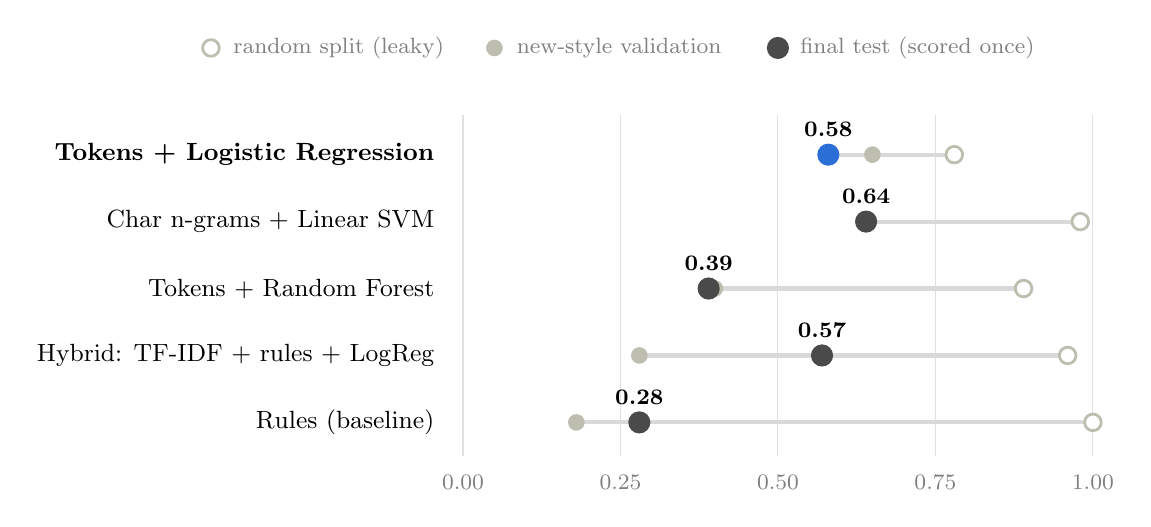
\begin{tikzpicture}[x=8cm, y=-0.85cm, font=\small]
  % axis
  \foreach \t in {0,0.25,0.5,0.75,1}{
    \draw[black!12] (\t,0.4) -- (\t,5.5);
    \node[text=gray, font=\footnotesize] at (\t,5.9) {\pgfmathprintnumber[fixed,precision=2,fixed zerofill]{\t}};
  }
  % rows: name / random / validation / test / chosen?
  \foreach \i/\name/\rnd/\val/\tst/\ch in {
      1/{\textbf{Tokens + Logistic Regression}}/0.78/0.65/0.58/1,
      2/{Char n-grams + Linear SVM}/0.98/0.64/0.64/0,
      3/{Tokens + Random Forest}/0.89/0.40/0.39/0,
      4/{Hybrid: TF-IDF + rules + LogReg}/0.96/0.28/0.57/0,
      5/{Rules (baseline)}/1.00/0.18/0.28/0}{
    \node[anchor=east] at (-0.03,\i) {\name};
    \pgfmathsetmacro{\lo}{min(\rnd,min(\val,\tst))}
    \pgfmathsetmacro{\hi}{max(\rnd,max(\val,\tst))}
    \draw[black!15, line width=1.5pt] (\lo,\i) -- (\hi,\i);
    \draw[muted, line width=1pt, fill=white] (\rnd,\i) circle (3pt);
    \fill[muted] (\val,\i) circle (3pt);
    \ifnum\ch=1
      \fill[accent] (\tst,\i) circle (4pt);
    \else
      \fill[dark] (\tst,\i) circle (4pt);
    \fi
    \node[font=\footnotesize\bfseries, above=3pt] at (\tst,\i) {\tst};
  }
  % legend
  \begin{scope}[yshift=0.25cm]
    \draw[muted, line width=1pt, fill=white] (-0.40,-0.3) circle (3pt);
    \node[anchor=west, font=\footnotesize, text=gray] at (-0.38,-0.3) {random split (leaky)};
    \fill[muted] (0.05,-0.3) circle (3pt);
    \node[anchor=west, font=\footnotesize, text=gray] at (0.07,-0.3) {new-style validation};
    \fill[dark] (0.50,-0.3) circle (4pt);
    \node[anchor=west, font=\footnotesize, text=gray] at (0.52,-0.3) {final test (scored once)};
  \end{scope}
\end{tikzpicture}
\caption{Macro-F1 over 9 classes for each model, measured three ways. Blue marks the model
the protocol chose: Logistic Regression scores 0.58 on the final test. Source:
\code{reports/results.json}; development set (199), new-style validation (63) and final
test (54).}
\label{fig:results}
\end{figure}

For the three pure machine-learning models, validation and test scores are within 0.07 of
each other, so the new-style validation set was a fair guide for them. The hybrid is the
exception: it scored 0.28 on validation and 0.57 on test, depending on how many rules
happen to fire on each set. The Linear SVM scored a little higher on test than the chosen
model (0.64 vs 0.58). It came second on validation, though (0.636 vs 0.646), and the
protocol does not allow switching after seeing test results. With 54 test snippets, a gap
of that size is not strong evidence either way. The random split again shows how leaked
templates inflate scores, to 0.78--1.00. In grouped cross-validation on the development
data, the rules still score 0.98, against 0.18 on validation and 0.28 on test.

\begin{table}[H]
\centering\small
\begin{tabular}{l r r r r}
\toprule
Model & Accuracy & Det.\ precision & Det.\ recall & Det.\ F1 \\
\midrule
\textbf{Tokens + Logistic Regression (chosen)} & \textbf{0.59} & \textbf{0.74} & \textbf{1.00} & \textbf{0.85} \\
Char n-grams + Linear SVM & 0.67 & 0.83 & 1.00 & 0.91 \\
Hybrid: TF-IDF + rules + LogReg & 0.57 & 0.83 & 0.62 & 0.71 \\
Tokens + Random Forest & 0.39 & 0.74 & 1.00 & 0.85 \\
Rules (baseline) & 0.41 & 1.00 & 0.28 & 0.43 \\
\bottomrule
\end{tabular}
\caption{Final test set, all metrics (54 snippets, 40 vulnerable). The chosen model is
first; the other rows are for transparency only.}
\end{table}

\begin{table}[H]
\centering\small
\begin{tabular}{l r r r r r}
\toprule
Class & Test snippets & Precision & Recall & F1 & Rules F1 \\
\midrule
LLM07 System prompt leakage & 6 & 1.00 & 1.00 & 1.00 & 0.67 \\
LLM03 Supply chain & 3 & 0.75 & 1.00 & 0.86 & 0.50 \\
LLM08 Vector store weaknesses & 6 & 0.75 & 1.00 & 0.86 & 0.00 \\
LLM05 Improper output handling & 6 & 0.60 & 1.00 & 0.75 & 0.00 \\
LLM01 Prompt injection & 6 & 0.67 & 0.67 & 0.67 & 0.00 \\
LLM06 Excessive agency & 3 & 0.43 & 1.00 & 0.60 & 0.00 \\
LLM10 Unbounded consumption & 5 & 0.31 & 0.80 & 0.44 & 0.89 \\
LLM02 Sensitive info disclosure & 5 & 0.00 & 0.00 & 0.00 & 0.00 \\
SAFE & 14 & 0.00 & 0.00 & 0.00 & 0.49 \\
\bottomrule
\end{tabular}
\caption{Per class on the test set: chosen model versus rules.}
\end{table}

Two problems stand out in the confusion matrix (\code{reports/figures/confusion\_test.png}):
\begin{itemize}
  \item \textbf{The model never predicts SAFE on new code.} All 14 safe test snippets are
        flagged, each as the risk its topic suggests: a filtered Milvus search becomes
        LLM08, a LangGraph agent with an approval step becomes LLM06. The model learned
        which topic a snippet is about, not whether the protection is present.
  \item \textbf{All 5 LLM02 snippets are predicted LLM10.} Data leaks through
        \code{serializers.serialize}, \code{analytics.track} or an error handler returning
        \code{process.env} look like ordinary endpoints to the model.
\end{itemize}

\subsection*{Examples predicted correctly (chosen model, test set)}

Prompt injection inside a class, using AWS Bedrock (never seen in training), predicted
\textbf{LLM01}:
\begin{lstlisting}[language=Python]
class ChatHandler:
    def run(self, user_query: str) -> str:
        body = json.dumps({"prompt": "Human: You work for Vandelay. " + user_query + " Assistant:",
                           "max_tokens_to_sample": 300})
        out = self.bedrock.invoke_model(modelId="meta.llama3-70b-instruct-v1:0", body=body)
\end{lstlisting}

A model-written SQL \code{WHERE} clause pasted into a pgvector query, predicted
\textbf{LLM05}:
\begin{lstlisting}[language=Python]
where = (await self.llm.ainvoke(f"Write only a SQL WHERE clause for: {ask}")).content
return await self.conn.fetch(f"SELECT * FROM users WHERE {where}")
\end{lstlisting}

A Redis vector search with no user filter, predicted \textbf{LLM08}. Secrets in a
YAML-loaded system prompt are predicted \textbf{LLM07}.

\subsection*{Examples predicted wrongly}

\textbf{Safe code with a tenant filter, true SAFE, predicted LLM08.} The filter is there,
but the words around it are the ones the model links to unsafe vector search:
\begin{lstlisting}[language=Python]
res = milvus.search(collection_name="documents", data=[embedder.embed(ask)], limit=5,
                    filter=f"account_id == {int(account_id)}", output_fields=["text"])
\end{lstlisting}

\textbf{Agent with a human approval step, true SAFE, predicted LLM06.}
The argument \code{interrupt\_before} is the safety control, but \code{refund} and
\code{create\_react\_agent} dominate:
\begin{lstlisting}[language=Python]
graph = create_react_agent(llm, tools=[lookup_order, refund], interrupt_before=["tools"],
                           checkpointer=MemorySaver())
\end{lstlisting}

\textbf{Card number sent to an analytics service, true LLM02, predicted LLM10.}
``card\_number'' and ``analytics.track'' never occur in training.

\textbf{User text inside a DSPy signature, true LLM01, predicted LLM05.}
\begin{lstlisting}[language=Python]
program = dspy.Predict(f"question -> answer; extra instructions: {ask}")
\end{lstlisting}

The errors share one cause: a bag-of-words model sees which words occur, not whether a
protection is present or how data flows. For the app this means many false alarms. That is
exactly what the planned LLM reviewer should catch, by reading each flagged function and
dismissing those that are already protected.

% =================================================================== 6
\section{Code, app and how to reproduce}

Everything above is reproducible from the repository
(\url{https://github.com/sovanpatricia/LLM-Security-Scanner}) in under a minute; the data
generators use fixed seeds and produce identical files on every run.

\begin{table}[H]
\centering\small
\begin{tabularx}{\linewidth}{>{\raggedright\arraybackslash}p{6.4cm} >{\raggedright\arraybackslash}X}
\toprule
Path & Content \\
\midrule
\code{data/build\_dataset.py}, \code{data/build\_val\_newstyle.py}, \code{data/build\_testset.py} & Template generators for the 199 development, 63 validation and 54 test snippets \\
\code{src/llmscan/rules.py} & The 34 baseline rules \\
\code{src/llmscan/features.py}, \code{models.py} & Comment stripping, code tokenizer, the four models and their grids \\
\code{experiments/run\_experiments.py} & EDA, tuning and model choice on validation, one final test, cross-validation, figures \\
\code{reports/} & \code{eda.json}, \code{results.json}, class-balance and confusion-matrix figures \\
\code{models/scanner\_model.joblib} & Logistic Regression (the chosen model) trained on development + validation \\
\code{src/llmscan/scan.py} & The app: a CLI that scans a file or folder \\
\bottomrule
\end{tabularx}
\caption{Repository layout.}
\end{table}

\textbf{The app.} The scanner splits each Python file into top-level functions and
assignments (with \code{ast}), and each TypeScript file into top-level declarations. It
keeps only units that touch an LLM and classifies each one with the chosen model. It then
prints a Markdown or JSON report with file, line, OWASP category, a score (the probability
of that label) and a suggested fix, plus a PASS/FAIL scorecard per category. It exits with
code 1 when it finds something and code 2 when the path does not exist, so it can block a
CI job. On the demo app \code{examples/vulnerable\_app.py}, it flags all three planted
bugs: the system prompt holding a password (LLM07), the shell command built by the model
(LLM05), and the \code{chat} endpoint, labelled LLM10 because it also has no token limit
(its f-string prompt makes LLM01 equally valid). It also flags the secure function
\code{safe\_answer} as LLM01, the same false-alarm problem seen on the test set. The app
replaces the hard-coded prediction from stage 1 with a real trained model.

\begin{lstlisting}[language=bash]
pip install -r requirements.txt
python experiments/run_experiments.py
PYTHONPATH=src python -m llmscan.scan examples/vulnerable_app.py
\end{lstlisting}

\subsection*{How the app works}

% ------------------------------------------------ scan flow
\begin{figure}[H]
\centering
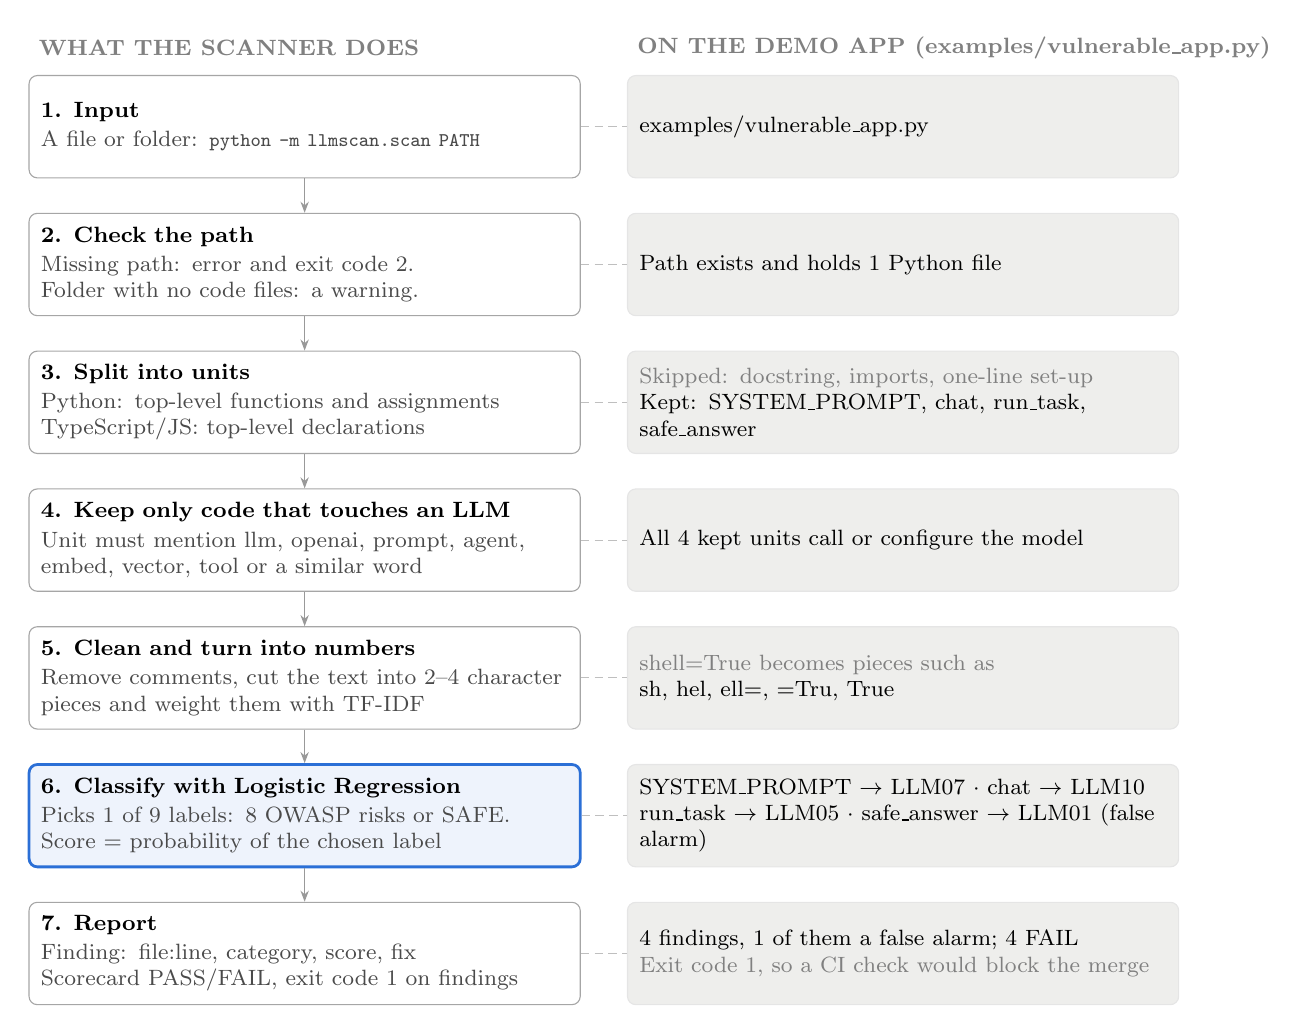
\begin{tikzpicture}[
    font=\footnotesize,
    stepbox/.style={draw=black!35, rounded corners=3pt, minimum width=7.0cm, minimum height=1.3cm,
                 align=left, text width=6.7cm, inner sep=4pt},
    ai/.style={stepbox, draw=accent, line width=1pt, fill=accent!8},
    demo/.style={fill=tint, draw=black!10, rounded corners=3pt, minimum width=7.0cm,
                 minimum height=1.3cm, align=left, text width=6.7cm, inner sep=4pt},
    arr/.style={-{Stealth[length=4pt]}, black!40},
    link/.style={black!25, densely dashed}
  ]
  \node[font=\footnotesize\bfseries, text=gray, anchor=west] at (-3.5,1.0) {WHAT THE SCANNER DOES};
  \node[font=\footnotesize\bfseries, text=gray, anchor=west] at (4.1,1.0) {ON THE DEMO APP (examples/vulnerable\_app.py)};

  \foreach \i/\hl/\title/\body/\demo in {
    1/0/{1. Input}/{A file or folder: {\ttfamily\scriptsize python -m llmscan.scan PATH}}/{examples/vulnerable\_app.py},
    2/0/{2. Check the path}/{Missing path: error and exit code 2.\\Folder with no code files: a warning.}/{Path exists and holds 1 Python file},
    3/0/{3. Split into units}/{Python: top-level functions and assignments\\TypeScript/JS: top-level declarations}/{\textcolor{gray}{Skipped: docstring, imports, one-line set-up}\\Kept: SYSTEM\_PROMPT, chat, run\_task, safe\_answer},
    4/0/{4. Keep only code that touches an LLM}/{Unit must mention llm, openai, prompt, agent,\\embed, vector, tool or a similar word}/{All 4 kept units call or configure the model},
    5/0/{5. Clean and turn into numbers}/{Remove comments, cut the text into 2--4 character\\pieces and weight them with TF-IDF}/{\textcolor{gray}{shell=True becomes pieces such as}\\sh, hel, ell=, =Tru, True},
    6/1/{6. Classify with Logistic Regression}/{Picks 1 of 9 labels: 8 OWASP risks or SAFE.\\Score = probability of the chosen label}/{SYSTEM\_PROMPT $\to$ LLM07 $\cdot$ chat $\to$ LLM10\\run\_task $\to$ LLM05 $\cdot$ safe\_answer $\to$ LLM01 (false alarm)},
    7/0/{7. Report}/{Finding: file:line, category, score, fix\\Scorecard PASS/FAIL, exit code 1 on findings}/{4 findings, 1 of them a false alarm; 4 FAIL\\\textcolor{gray}{Exit code 1, so a CI check would block the merge}}
  }{
    \ifnum\hl=1 \def\sc{accent}\def\sf{accent!8}\def\lw{1pt}\else \def\sc{black!35}\def\sf{white}\def\lw{0.4pt}\fi
    \node[stepbox, draw=\sc, fill=\sf, line width=\lw] (s\i) at (0,-1.75*\i+1.75) {\textbf{\title}\\[1pt]{\color{dark}\body}};
    \node[demo] (d\i) at (7.6,-1.75*\i+1.75) {\demo};
    \draw[link] (s\i.east) -- (d\i.west);
  }
  \foreach \i [evaluate=\i as \j using int(\i+1)] in {1,...,6}{
    \draw[arr] (s\i.south) -- (s\j.north);
  }
\end{tikzpicture}
\caption{Scan flow: the scanner turns each function into a label in seven steps, shown on
\code{examples/vulnerable\_app.py}.}
\label{fig:scan}
\end{figure}

Only step 6 uses AI. Steps 1--5 prepare the code so the model sees one function at a time,
and step 7 turns the labels into a report. The scores are low (0.13--0.15) because the
chosen model is strongly regularised ($C = 0.1$), which spreads probability across the 9
labels. Read them as a ranking, not as a confidence.

% ------------------------------------------------ training flow
\begin{figure}[H]
\centering
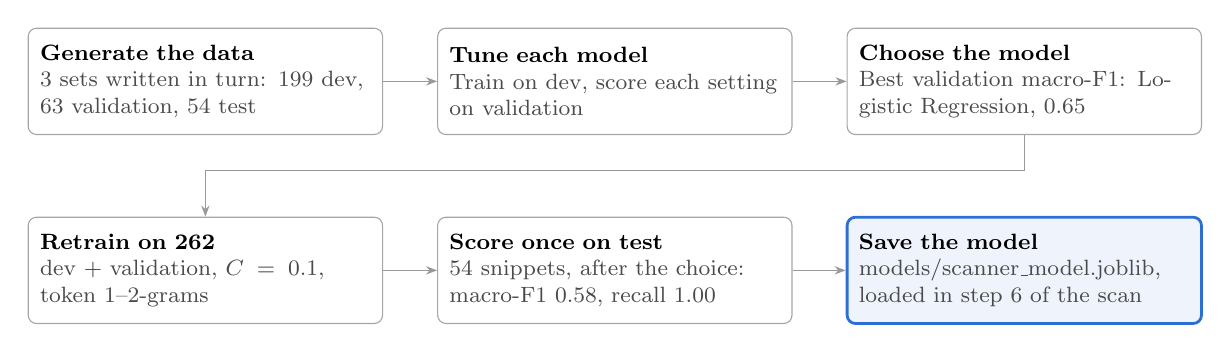
\begin{tikzpicture}[
    font=\footnotesize,
    box/.style={draw=black!35, rounded corners=3pt, minimum width=4.5cm, minimum height=1.35cm,
                align=left, text width=4.2cm, inner sep=4pt},
    final/.style={box, draw=accent, line width=1pt, fill=accent!8},
    arr/.style={-{Stealth[length=4pt]}, black!40}
  ]
  \node[box]   (a) at (0,0)      {\textbf{Generate the data}\\{\color{dark}3 sets written in turn: 199 dev, 63 validation, 54 test}};
  \node[box]   (b) at (5.2,0)    {\textbf{Tune each model}\\{\color{dark}Train on dev, score each setting on validation}};
  \node[box]   (c) at (10.4,0)   {\textbf{Choose the model}\\{\color{dark}Best validation macro-F1: Logistic Regression, 0.65}};
  \node[box]   (d) at (0,-2.4)   {\textbf{Retrain on 262}\\{\color{dark}dev + validation, $C = 0.1$, token 1--2-grams}};
  \node[box]   (e) at (5.2,-2.4) {\textbf{Score once on test}\\{\color{dark}54 snippets, after the choice: macro-F1 0.58, recall 1.00}};
  \node[final] (f) at (10.4,-2.4){\textbf{Save the model}\\{\color{dark}models/scanner\_model.joblib, loaded in step 6 of the scan}};
  \draw[arr] (a) -- (b);
  \draw[arr] (b) -- (c);
  \draw[arr] (c.south) -- ++(0,-0.45) -| (d.north);
  \draw[arr] (d) -- (e);
  \draw[arr] (e) -- (f);
\end{tikzpicture}
\caption{Training flow (\code{experiments/run\_experiments.py}): the model is chosen on
validation, retrained, then tested once.}
\label{fig:train}
\end{figure}

Training happens once, with \code{python experiments/run\_experiments.py}; scanning
reuses the saved file and takes under a second. The test set plays no part in the choice:
it is scored only after the model is fixed.

\end{document}
